\documentclass{dithesis}
\usepackage{mathspec}
\usepackage{xgreek}
\usepackage{xunicode}

% Math
\usepackage{amsfonts}

% Tikz
\usepackage{tikz}
\usetikzlibrary{arrows}
\usepackage{smartdiagram}
\usetikzlibrary{mindmap}
\usetikzlibrary{trees}

% Images
\usepackage{graphicx}
\graphicspath{ {images/} }

% Code
\usepackage{listings}
\usepackage{minted}

% URL
\usepackage{url}

\setallmainfonts[Mapping=tex-text]{Arial}
\setallsansfonts[Mapping=tex-text]{Arial}
\setallmonofonts[Mapping=tex-text]{Arial}

\renewcommand{\university}{National and Kapodistrian University of Athens}
\renewcommand{\school}{Faculty of Exact Sciences}
\renewcommand{\department}{Department of Informatics and Telecommunications}
\renewcommand{\thesisplace}{Athens}
\renewcommand{\thesisdate}{April 2016}
\renewcommand{\thesislabel}{Bachelor Thesis}
\renewcommand{\supervisorlabel}{Supervisors}
\renewcommand{\idlabel}{Α.Μ.}

\renewcommand{\contentsname}{Contents}
\renewcommand{\listfigurename}{List of Figures\vspace{5 mm}}
\renewcommand{\figurename}{Figure}
\renewcommand{\listtablename}{List of Tables\vspace{5 mm}}
\renewcommand{\tablename}{Table}
\renewcommand{\refname}{References}

\begin{document}
\thesistitle{RHEA: A Reactive, Heterogeneous, Extensible and Abstract Framework for Dataflow Programming}
\thesisauthor{Orestis Melkonian}{1115201000128}
\supervisor{Panos Rondogiannis}{Professor EKPA}
\supervisor{Angelos Charalambidis}{Researcher NCSR}
\maketitle

\begin{thesisabstract}[Abstract]
Summary here

\thesiskeywords
{Subject Area}{Programming Languages}
{Keywords}
	{dataflow}
	{stream}
	{frp}
	{distributed systems}
	{model-driven architecture}
	{program synthesis}
	{declarative languages}
	{node placement}
\end{thesisabstract}

\begin{thesisdedication}
"τὰ όντα ιέναι τε πάντα καὶ μένειν ουδέν" \\
(all entities move and nothing remains still) \\
- Heraclitus
\end{thesisdedication}

\begin{thesisacknowledgments}[Acknowledgements]

I would like to thank Angelos Charalambidis for his immensely helpful supervision and guidance throughout the whole period of 6 months that I was present in NCSR. 

I would also like to thank Professor Panos Randogiannis for being a major influence in my current research interests through the undergraduate courses "Theory of Computation" and "Principles of Programming Languages", where I was introduced to a much more declarative way of programming and started appreciating mathematical sensibility in computing.

\end{thesisacknowledgments}

\tableofcontents
\listoffigures

\begin{thesisprologue}[Prologue]

This bachelor thesis is a continuation of my internship at the National Centre for Scientific Research "Demokritos", particularly in the Software and Knowledge Engineering Laboratory (SKEL). 

The main task I was assigned was the implementation of a framework for robot programming using a dataflow approach. During that internship, I came to realize that my work could be easily generalized to cover a much broader application area than just robot software. 

The name of the framework stems from the ancient Greek Titaness Rhea(\textit{Ρέα}), daughter of earth goddess Gaia(\textit{Γαία}) and sky god Uranus(\textit{Ουρανός}) and etymologically derives from the verb \textit{ρέω}(to flow).

\end{thesisprologue}


\thesissection{Introduction}

\thesissubsection{Main concept}

My main contribution is the design and implementation of a framework for dataflow programming to be deployed anywhere, ranging from low-performance robots and sensors to clusters of computer and even the Cloud. 

The main idea is to provide the programmer with a different execution model, the dataflow model, which allows for a more abstract way of thinking and has the advantage of exposing opportunities for parallelism (amongst CPU cores) and distribution (amongst computational machines) that the "intelligent" underlying system can automatically realize. Therefore, the programmer will be able to gain good performance and utilization of the available computational resources, while at the same time reducing development time and cost and maintaining a much cleaner and easier-to-refactor software system.


\thesissubsection{Motivation}

\thesissubsubsection{Declarative languages}

Software is becoming increasingly more complex each year, as computing capabilities are strengthened and user needs become more and more demanding. Thus the need for higher abstraction becomes mandatory, as it provides a more structured, easier to debug and maintainable way of developing software. In other words, abstraction in computer science acts as a mean to overcome complexity. 

In programming languages, the level of the aforementioned abstraction is measured regarding the amount of low-level details a programmer has to specify. Therefore, languages can be divided in two categories: the imperative ones, which specify what needs to be done and how to do it, and the declarative ones, which only specify what needs to be done and rely on the underlying compiler/interpreter to produce the exact commands that will realize the desired behaviour. The most well-known declarative programming paradigms are functional and logic programming, each providing higher abstraction in different aspects. My approach was greatly influenced by the functional paradigm.

\thesissubsubsection{Data versus Computation}			

A common problem in heterogeneous systems is that different representations of the same entities/data-types coexist in the same software and, as a consequence, pure computational tasks are intermingled with data-converting tasks. This makes the code less readable and harder to maintain and understand. In the dataflow execution model, there is a clear separation of these two aspects as data (edges) are completely decoupled from computation (nodes). This motivation is strengthened even more, when cross-machine communication is included, and apart from converting data from one representation to another, serialization(i.e. convertion to bytes) is also mandatory.

\thesissubsubsection{Dataflows in Robotics}

In control theory, which is the main background theory used in robotics, most architectures and/or algorithms are represented as dataflow diagrams for the sake of clarity and intuition. Translating these diagrams into common "imperative" software is not an easy tasks and is usually the source of bugs. Thus, having a dataflow execution model will nullify the need for such a translation.

Moreover, robotics typically involve several different robotic systems, whose combination is even more challenging. If each individual system is represented as a dataflow graph, composing them together is as trivial as connecting inputs with outputs, which is not the case in a traditional architecture, which is not component-based.

\thesissubsubsection{Dataflows in Big Data}

Another reason for following a dataflow approach is the attention that it recently has drawn in the Big Data field. As data size is growing exponentially and distribution is not a luxury but a necessity, a more scalable and decentralized architecture was destined to be examined in more depth. As we will discuss in the \textit{Related Work} chapter, there are many recent frameworks that became popular for the scalability due to the fact that they rely on a dataflow approach.

\thesissubsection{Outline}

There are nine chapters which compose this thesis: \textit{Introduction, Background, Approach, Implementation, Applications, Related Work, Future Work, Conclusions}.

\textit{Background} introduces the reader to basic background knowledge, necessary for complete understanding.

\textit{Approach} presents the main characteristics of my approach.

\textit{Implementation} gives a more detailed specification of the framework.

\textit{Applications} present some use-cases, ranging from general mathematical problems to real-life robot scenarios.

\textit{Related Work} discusses relevant concepts and technologies, which influenced major decisions concerning the design and implementation of the framework.

\textit{Future Work} suggests some interesting topics for future research, whose embedding in the framework is meaningful.

\textit{Conclusions} sums up.

\thesissection{Background}

\thesissubsection{The dataflow computational model}
The increased interest in parallelism during the 70's gave rise to the dataflow execution model, which is an alternative to the classical "von-Neumann" model. In the dataflow model, everything is represented in a dataflow graph, where nodes are independent computational units  and edges are communication channels between these units. A node/unit is fired immediately when its required inputs are available and therefore no explicit control commands are needed for execution. Figure 1 shows a dataflow graph enumerating the set $\mathbb{N}$ of natural numbers.

\begin{figure}[h!] \begin{center} 
	\begin{tikzpicture}[
  every matrix/.style={ampersand replacement=\&,column sep=3cm,row sep=2cm},
  source/.style={draw,thick,rounded corners,inner sep=.3cm,fill=yellow!20},
  process/.style={source,fill=cyan!20},
  sink/.style={source,fill=green!20},
  to/.style={->,>=stealth',shorten >=1pt,semithick},
  every node/.style={align=center}]

  \matrix{
    \& \node[source] (zero) {0};
    \& \node[process] (concat) {concat}; 
    \& \node[sink] (res) {$\mathbb{N}$}; \\
    \& \& \node[process] (inc) {increment}; \& \& \\
  };
  \draw[to] (zero) -- (concat);
  \draw[to] (concat) -- (res);
  \draw[to] (concat) to[bend left=50] (inc);
  \draw[to] (inc) to[bend left=50] (concat);
\end{tikzpicture} 	
	\caption{Natural numbers}
\end{center} \end{figure}


The main advantage of the dataflow model is its implicit parallelism, deriving from the fact that the computational units are totally independent and therefore can be executed in parallel. The communication can either be an in-memory data storage or even a TCP connection across the network. Its great flexibility and composability make it a good candidate for the underlying architecture of a framework with a high level of abstraction.

\thesissubsection{Functional reactive programming}
A relatively recent model of programming is Functional Reactive Programming (FRP), which provides a conceptual framework for implementing reactive(i.e. time-varying and responding to external stimuli) behaviour in \textit{hybrid systems} (i.e. containing both continuous and discrete components), such as robots, in functional programming languages. It first appeared as a composable library for graphic animations \cite{fran}, but quickly evolved into a generic paradigm \cite{survey_frp,real_frp,pushpull_frp}. Moreover, extensive research has investigated FRP as a framework for robotics \cite{arrows_robots,lambda_in_motion}. \\
Although appealing at first, FRP was not appropriate for systems  with real-time constraints, due to uncontrollable time- and space- leaks \cite{event_frp}. The solution was a generalization of monads called \textit{arrows} \cite{arrows}, which provided the necessary guarantees that the aforementioned common errors do not occur. Let's see the example of calculating a robot's x-coordinate. Here is the mathematical formula drawn from control theory:

$$ x = 1/2 \int (vr + vl) \cos\theta $$ 

Below is the FRP code corresponding to the formula above:

\newmintedfile[hs]{hs}{frame=lines}
\usemintedstyle{bw }
\hs{code/frp1.hs}

As the above may seem counter-intuitive, a new notation was conceived, notably the \textit{arrow notation} \cite{arrows_notation}:

\hs{code/frp2.hs}

The main advantages of FRP are its close correspondence to mathematics, which make it an ideal framework for modelling real-time systems, and its concise representation of time-varying values via \textit{signals}. \\
For a more detailed view of the FRP idiom and all of its variants please see the cited literature.

\thesissubsection{Publish-Subscribe model}

\textit{Publish/Subscribe}(PubSub) is a communication paradigm that became popular due to the loose coupling of its components, suited for the most recent large-scale distributed applications.

There is no point-to-point communication and no synchronization. \textit{Publishers} advertise messages of a given type to a specific message class or \textit{topic} that is identified by a \textit{keyword}, whereas \textit{subscribers} listen on a specific \textit{topic} without any knowledge of who the publishers are. The component responsible for relaying the messages between machines and/or processes and finding the cheaper dissemination method is called \textit{message broker}. Figure 2 illustrates an abstract representation of the PubSub model.

\begin{figure}[h!] \begin{center}    
  	\begin{tikzpicture}
      % Publishers
      \draw [red,fill] (-2.5,0) circle [radius=0.2] node [black,left=4] {Publisher};
      \draw [red,fill] (-2.5,1) circle [radius=0.2] node [black,left=4] {Publisher};
      \draw [red,fill] (-2.5,2) circle [radius=0.2] node [black,left=4] {Publisher};

      % Broker
      \draw [fill] (-0.2,0.5) rectangle (0.2, 1.5) node [black,below=-15] {Broker};
      
      % Subscribers
      \draw [orange,fill] (2.5,0.5) circle [radius=0.2] node [black,right=4] {Subscriber};
      \draw [orange,fill] (2.5,1.5) circle [radius=0.2] node [black,right=4] {Subscriber};
      
      % Edges
      \draw [thick] (-2.5,0)
      to [out=10,in=190] (0,1)
      to [out=10,in=190] (2.5,0.5); 
      \draw [thick] (-2.5,2)
      to [out=10,in=170] (0,1)
      to [out=10,in=190] (2.5,1.5);
      \draw [thick] (-2.5,1) to (0,1);       
\end{tikzpicture} 
  	\caption{PubSub typical layout}
\end{center} \end{figure}

\thesissubsection{ROS: Robot Operating System}

ROS is an open-source middleware for robot software, which emphasizes large-scale integrative robotics research \cite{ROS}. It provides a \textit{thin} communication layer between heterogeneous computers, from robots to mainframes and tt has been widely adopted by the research community around the world, due to its flexibility and maximal support of reusability through packaging and composability. It provides a nice solution to the development complexity introduced by complex robot applications that consist of several modules and require different device drivers for each individual robot. 

It follows a peer-to-peer network topology, implemented using a topic-based PubSub messaging protocol and its architecture reflects many sound design principles. Another great property of ROS is that it is language-agnostic, meaning that only a minimal specification language for message transaction has been defined, so contributors are free to implement small-size clients in different programming languages, with \textit{roscpp} and \textit{rospy} being the most widely used ones.

A typical development scenario is to write several \textit{nodes}, that subscribe to some topics and, after doing some computation, publish their results on other topics. The main architectural issue here is that subscribing is realized through asynchronous callback functions, so complicated schemes easily lead to unstructured code, which obviously lead to unreadable and hard-to-maintain code. My approach gives a solution to the aforementioned problem.
 
\thesissubsection{Internet of things}

The birth of the Internet gave rise to a concept called \textit{Internet of Things} (IoT), which is essentially the ability of many heterogeneous devices, ranging from low-cost sensors to vehicles with embedded electronics, to collect data and exchange it amongst themselves using the Internet. This gave rise to smart grids, smart homes and eventually smart cities. 

The development of such systems though, due to their heterogeneity, is rather complex and costly. Typical software architectures were not meant to be used in such environments and therefore new tools and concepts needed to be invented. 

Fortunately, the dataflow model seems to be rather fitting for these scenarios, as every node in the graph is completely independent, and consequently can be any "\textit{thing}". This useful property of the model makes it a good architectural choice for such applications. The only thing to consider is how these things will communicate in a standard way, so as to be able to add new types of \textit{things} and integrate it in an effortless way to an existing dataflow network of \textit{things}.

\thesissubsection{The Strategy design pattern}

In software engineering, and especially in object-oriented programming(OOP), a \textit{design pattern} is a general repeatable solution to a commonly occurring problem in software design \cite{design}.

One such solution, the \textit{Strategy} design pattern is used when a particular algorithm can be implemented by a variety of behaviours/classes \cite{design}. In such a case, a good idea is to isolate the algorithm in a separate \textit{interface} and allow the system to select the appropriate instantiating classes at runtime.

Figure 3 illustrates the basic UML diagram of the strategy design pattern.

\begin{figure}[h!] \begin{center}    
	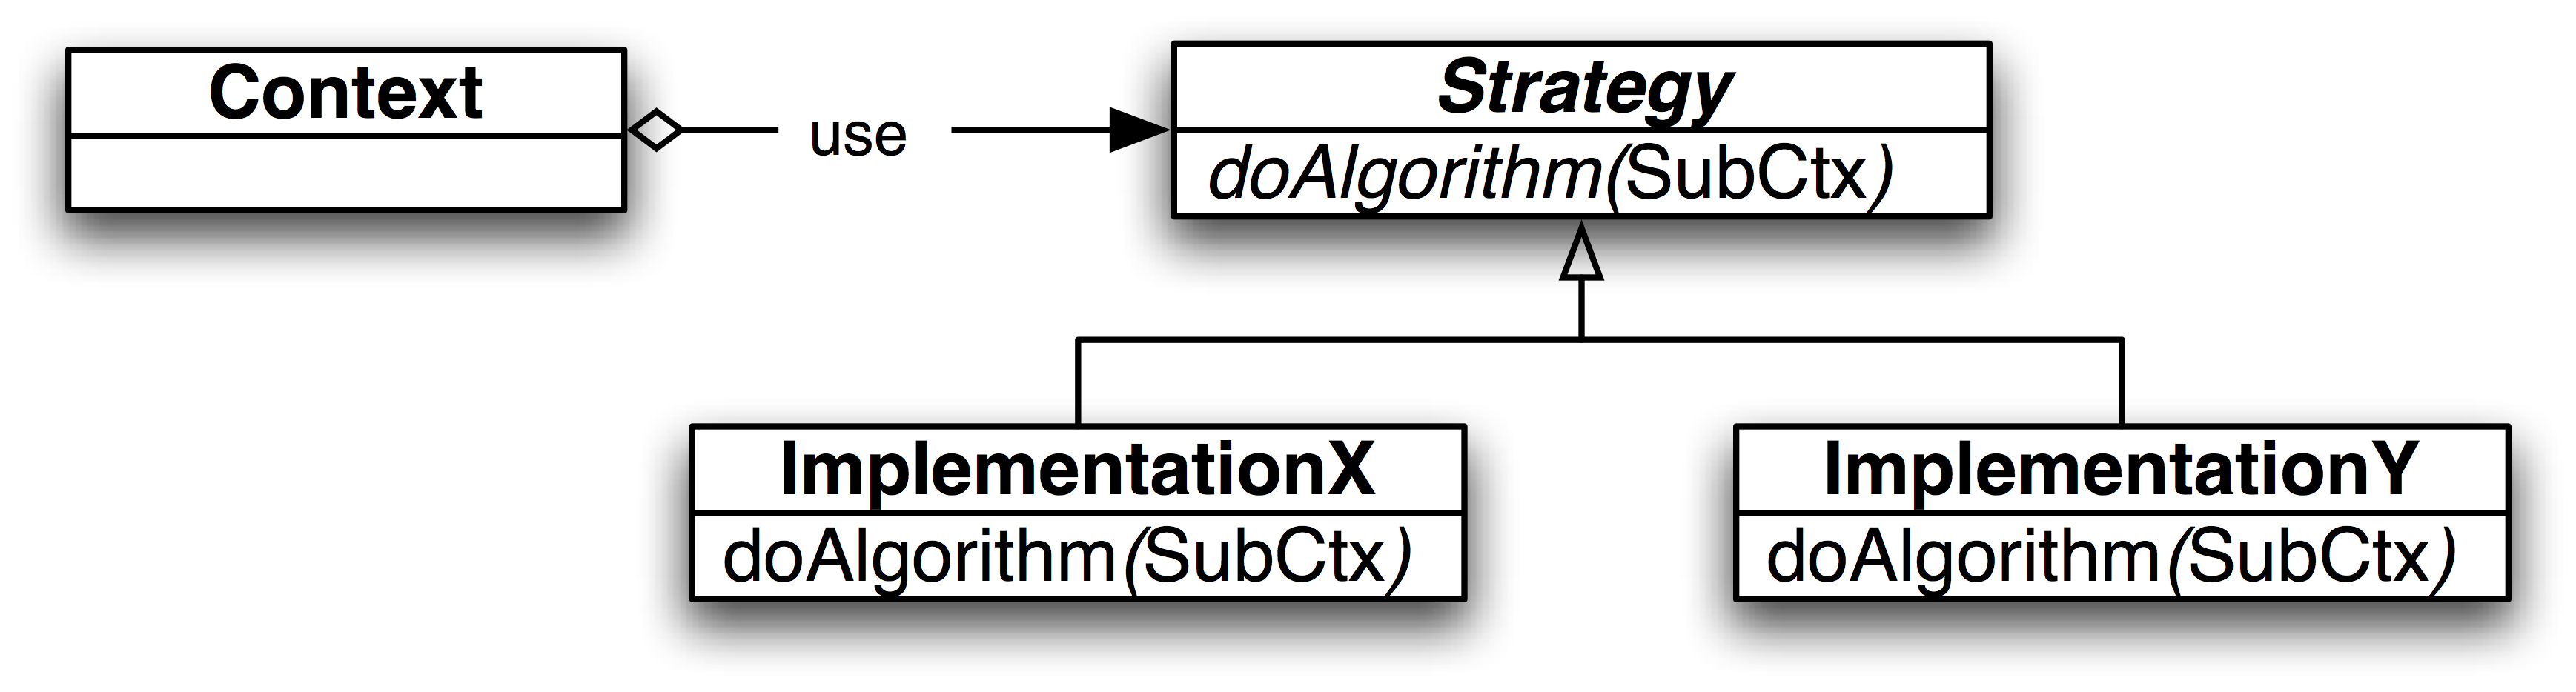
\includegraphics[scale=0.1]{strategy}
  	\caption{Strategy design pattern}
\end{center} \end{figure}

\thesissection{Approach}
The design was heavily influenced by principles set out by the FRP and dataflow models. 

\thesissubsection{Reactive}

The system is \textit{reactive}, as close as possible to the definition of the Reactive Manifesto \cite{manifesto}. 

The system is \textit{responsive}, meaning it should be able to handle time-sensitive scenarios if at all possible. This is the cornerstone of usability and utility, but more than that, it enables quick error-detection and error-handling.

The system is \textit{resilient}, meaning it is able to recover robustly and gracefully after a failure, due to the fact that nodes in the dataflow graph are completely independent and recovery of each one can be done in textit{isolation}. Another thing to note here is that special error messages are built-in and make it very easy to propagate errors between \textit{components}, in case the error-handling part of a component is decoupled from the computational logic. This leads to much more robust architectures for large-scale systems, where fault-tolerance is mission-critical.

The system is \textit{elastic}, meaning it will adjust itself depending on the available resources and demanded workload. For instance, the granularity of the graph (i.e. number of nodes) is adjusted so as to match a heuristic-based value (e.g. total number of threads).

The system is \textit{message-driven}, meaning it relies solely on asynchronous message-passing for inter-component communication leading to loose coupling, isolation, location transparency and the error propagation mentioned above. Location transparency is critical to preserve the semantics whether on a single host or a machine cluster. 

\begin{figure}[h!] \begin{center}    
  	\smartdiagramset{bubble center node size = 40mm, bubble node size = 25mm}
\smartdiagram[bubble diagram]
{
  reactive,
  responsive, resilient, elastic, message\\driven
}
 
  	\caption{Reactive properties}
\end{center} \end{figure}

\thesissubsection{Heterogeneous}

One of the major concerns while designing the framework was the ability to deploy it anywhere, from low-cost robots to mainframes. Obviously, such attribute would require a very flexible runtime environment. To satisfy this requirement, the strategy design pattern was used for evaluation, meaning that the core system only builds the internal representation of the dataflow graph and partitions it across the available computational resources. From there onwards, each partial graph can be evaluated by a different \textit{EvaluationStrategy} (see Implementation chapter), which could interpret it using the Java 8 Streams library or even compile into CUDA code for execution on a GPU.

Figure 5 illustrates a simple example of a robot application pipeline, where input to the dataflow graph is what the robot's camera senses, and after some image processing and some computation-heavy decision making, a command to an actuator of the robot is executed. Orange nodes are deployed on the robot's on-board computer, the green node is deployed on an off-board GPU and the red node is deployed on the lab's main cluster.

\begin{figure}[h!] \begin{center}    
 	\begin{tikzpicture}[
  mindmap, concept color=orange,
  level 1/.append style={level distance=3cm},
  level 2/.append style={level distance=3cm},
  level 3/.append style={level distance=3cm},
  level 4/.append style={level distance=3cm}
  ]
  \tikzset{every concept/.style={minimum size=2cm, text width=2cm}} 
  \tikzstyle{every node}=[font=\small]
  \node[concept] {robot\\camera}
    child[concept color=orange, grow=right]{ node[concept]{compress}
      child[concept color=green, grow=right]{ node[concept]{image\\processing} 
        child[concept color=red, grow=right]{  node[concept]{decision}
          child[concept color=orange, grow=right]{ node[concept]{robot\\command} } 
        } 
      }
    }; 

\end{tikzpicture} 
  	\caption{Heterogeneity pipeline}
\end{center} \end{figure}

\thesissubsection{Extensible}

While doing my internship at NCSR "Demokritos", I realized that the goal I was pursuing was impossible to reach closure in a 6-month period by a humble undergraduate student. Therefore, I decided that everything should be implemented in a way that will allow future contribution by me or other researchers/developers. 

With that concept in mind, I started generalizing and abstracting away everything I had done so far with the hope that the framework will raise attention later on. I can now say I am satisfied with the level of abstraction the core system has reached and I hope the stressful refactoring that the framework went through will blossom in the form of future contributions.

\thesissubsection{Abstract}

The framework is \textit{abstract} in terms of implementation details, as it is completely agnostic of any machine-specific or runtime-specific requirements. It is designed as a unifying conceptual base for further refined extensions and careful consideration was taken not to restrict in any aspect, architectural or not. The above was achieved by making many parts of the core system pluggable, which allows for easy refactoring on most of its internal functionality.

\thesissection{Implementation}

\thesissubsection{The Reactive Streams Standard}

\thesissubsection{Stream variables}

\thesissubsection{Stream operators}
\thesissubsubsection{Creation}
\thesissubsubsection{Combining}
\thesissubsubsection{Filtering}
\thesissubsubsection{Conditional}
\thesissubsubsection{Transformational}
\thesissubsubsection{Feedback}
\thesissubsubsection{Error-handling}
\thesissubsubsection{Backpressure}
\thesissubsubsection{Utility}

\thesissubsection{Deployment}


\thesissubsection{Optimization}

\thesissubsubsection{Heuristic-based graph transformations}
\thesissubsubsection{Network-aware node placement}


\thesissubsection{Serialization}


\thesissection{Applications}

\thesissubsection{Hamming numbers}
\thesissubsection{Camera surveilance}
\thesissubsection{Robot control panel}
\thesissubsection{Robot hospital guide}

\thesissection{Related Work}

\thesissubsection{Big Data}
\thesissubsubsection{GoogleDataflow}
\thesissubsubsection{TensorFlow}
\thesissubsubsection{Akka}
\thesissubsubsection{dispel4py}
\thesissubsubsection{Spark}
\thesissubsubsection{Naiad}

\thesissubsection{Robotics}
\thesissubsubsection{Flowstone}
\thesissubsubsection{Yampa}
\thesissubsubsection{roshask}

\thesissubsection{Internet of Things}
\thesissubsubsection{NodeRed}
\thesissubsubsection{NoFlo}

\thesissection{Future Work}

\thesissubsection{More evaluation strategies}
\thesissubsection{Dynamic reconfiguration}
\thesissubsection{Advanced network profiling}
\thesissubsection{DSLs for framework extension}
\thesissubsection{Advanced fault-tolerance}
\thesissubsection{Integration with other technologies}
\thesissubsection{Stream reasoning}

\thesissection{Conclusions}

\begin{thesisterminology}
A table of used scientific terms follows.

\begin{tabularx}{\textwidth}{|X|X|}
  \hline
  κλάσση & class \\
  \hline
  εντολή & command \\
  \hline
  περιβάλλον & environment \\
  \hline
\end{tabularx} 
\end{thesisterminology}

\begin{thesisabbreviations}
A table of all abbrevations used throughout the thesis follows.

\begin{tabularx}{\textwidth}{|X|X|}
  \hline
  FRP & Functional Reactive Programming \\
  JVM & Java Virtual Machine \\
  NCSR & National Centre for Scientific Research \\
  ROS & Robot Operating System \\
  IoT & Internet of Things \\
  CPU & Central Processing Unit \\
  TCP & Transmission Control Protocol \\
  PubSub & Publish/Subscribe \\
  OOP & Object-oriented Programming \\
  UML & Unified Modelling Language \\
  GPU & Graphics Processing Unit \\
  DSL & Domain-specific Language \\
  \hline
\end{tabularx}

\end{thesisabbreviations}

\newpage
\bibliographystyle{ieeetr}
\bibliography{thesis}{}

\end{document}
